\section{Multigrid Methods}
Multigrid methods have been designed to accelerate the convergence of iterative methods by eliminating certain error components on a so-called coarser representation of the original problem.
While the basic iterative methods discussed in the last section are applicable to many PDE-based problems, in practice, their speed of convergence is often insufficient, which means that a large number of iterations is required until an acceptable approximation accuracy can be attained. 
The main reason for this behavior is that these methods are only efficient in the reduction of certain error components, while others remain mostly unaffected~\cite{briggs2000multigrid}.
This can be best understood by considering the effect of a stationary iterative method on oscillatory errors of different frequency.
For this purpose, we consider the one-dimensional Laplace equation
\begin{equation}
		\begin{split}
			- \dv[2]{x} u(x) & = 0 \quad \forall x \in (0, 1) \\
			u(0) = u(1) & = 0,
		\end{split}
		\label{eq:1D-laplace-model}
\end{equation}
which is discretized using the three-point stencil
\begin{equation}
	\Delta_h^{(3, 1)} = \frac{1}{h^2}\begin{bmatrix}
		-1 & 2 & -1
	\end{bmatrix}.
		\label{eq:1D-laplace-stencil}
\end{equation} 
Figure~\ref{fig:different-error-components} shows the impact of applying the Jacobi´and Gauss-Seidel method on different periodic error components.
\begin{figure}
	\centering
	\begin{subfigure}[b]{0.32\textwidth}
		\centering
		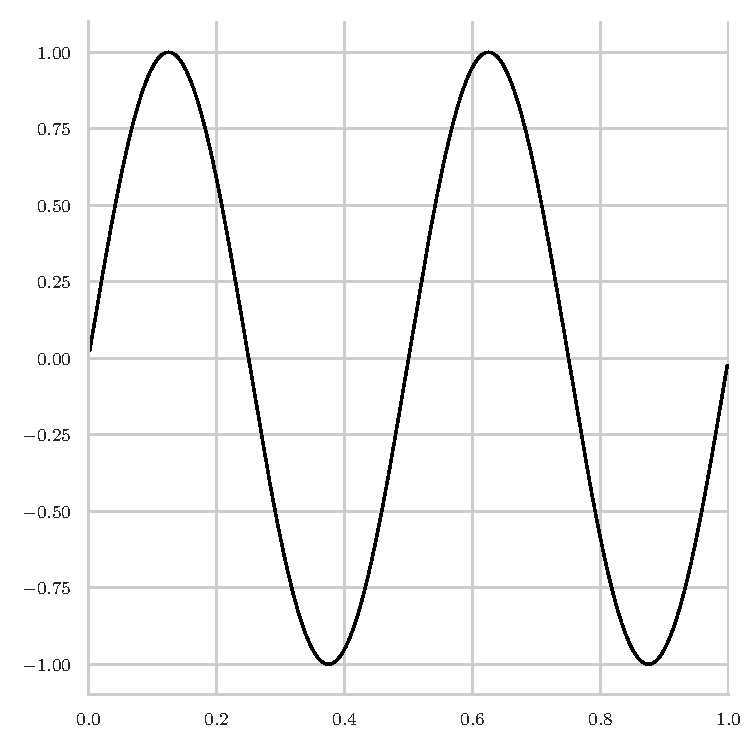
\includegraphics[width=\textwidth]{figures/initial_error_jacobi_4pi.pdf}
		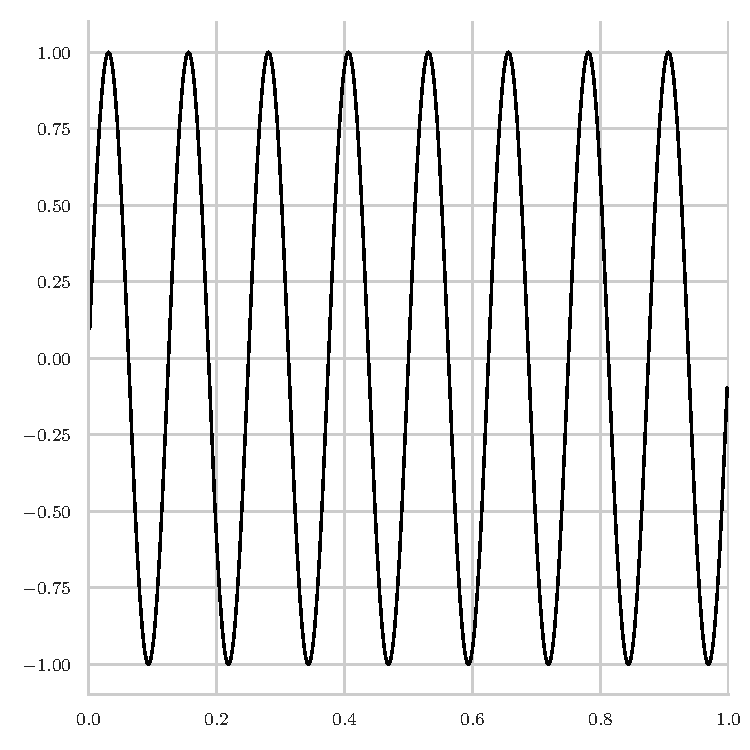
\includegraphics[width=\textwidth]{figures/initial_error_jacobi_16pi.pdf}
		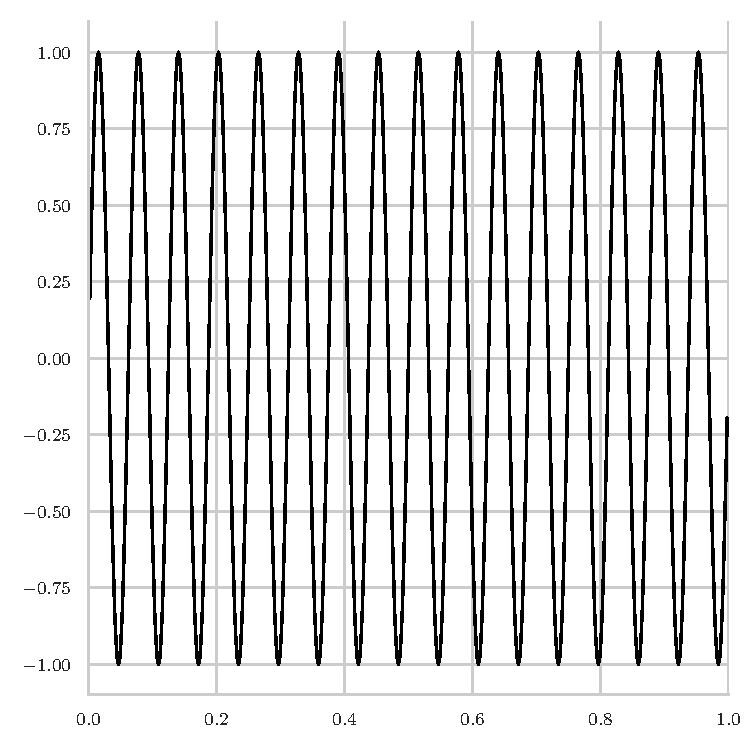
\includegraphics[width=\textwidth]{figures/initial_error_jacobi_32pi.pdf}
		\caption{Initial error}
	\end{subfigure}
	\hfill
	\begin{subfigure}[b]{0.32\textwidth}
		\centering
		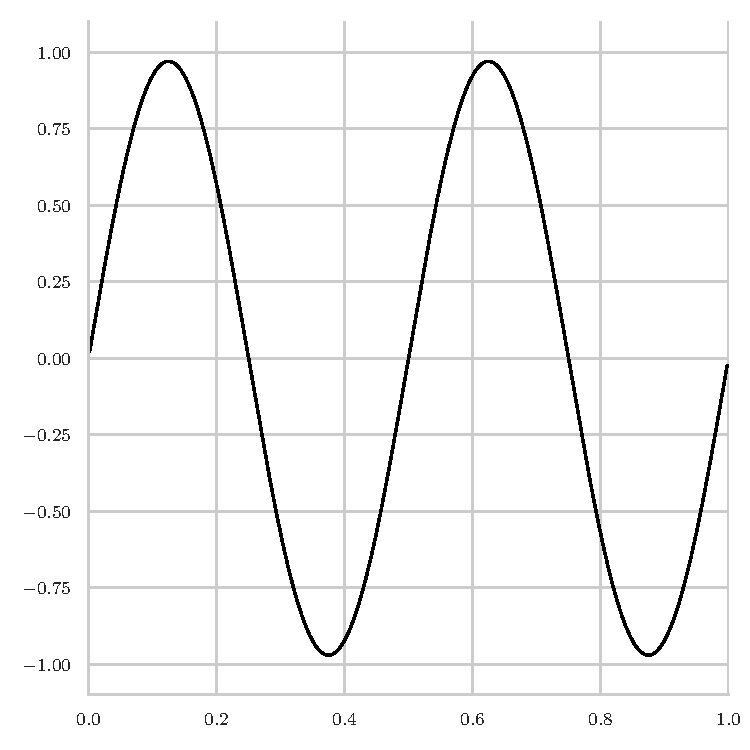
\includegraphics[width=\textwidth]{figures/final_error_jacobi_4pi.pdf}
		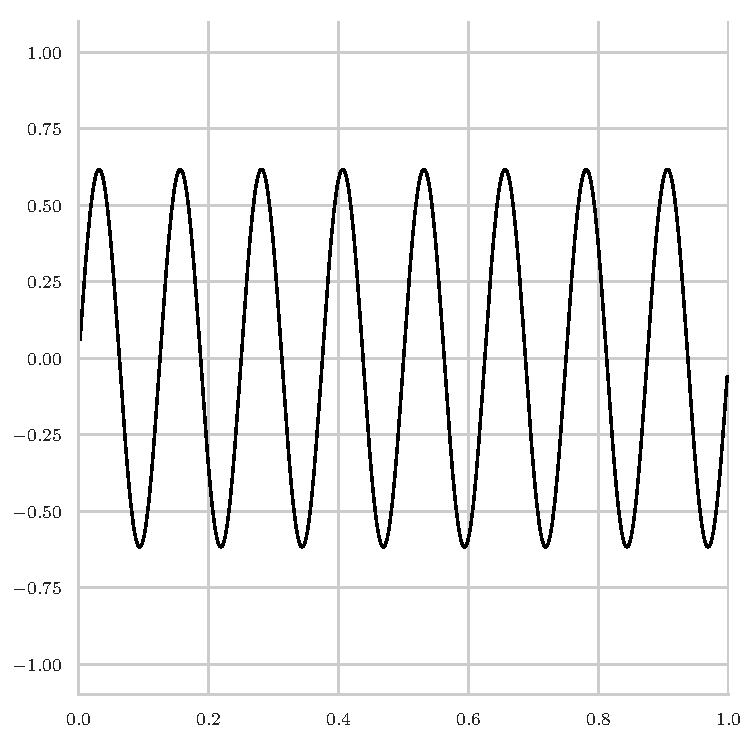
\includegraphics[width=\textwidth]{figures/final_error_jacobi_16pi.pdf}
		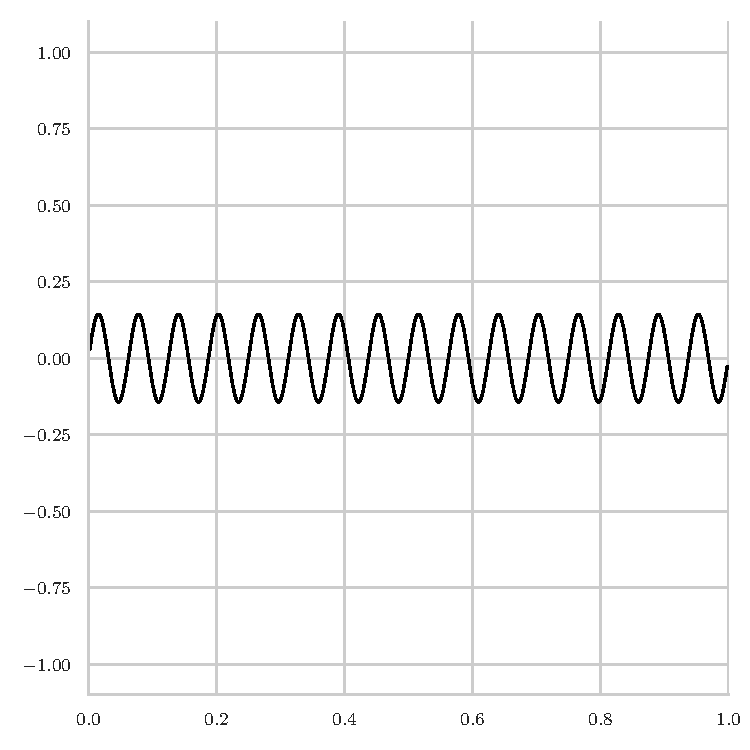
\includegraphics[width=\textwidth]{figures/final_error_jacobi_32pi.pdf}
	\caption{Error after applying Jacobi}
	\end{subfigure}
	\hfill
	\begin{subfigure}[b]{0.32\textwidth}
		\centering
		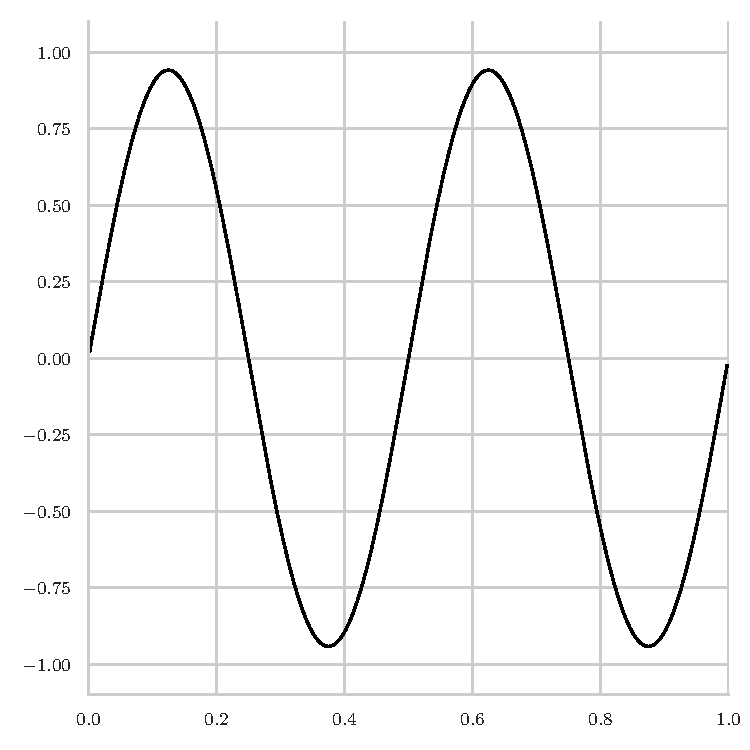
\includegraphics[width=\textwidth]{figures/final_error_gauss_seidel_4pi.pdf}
		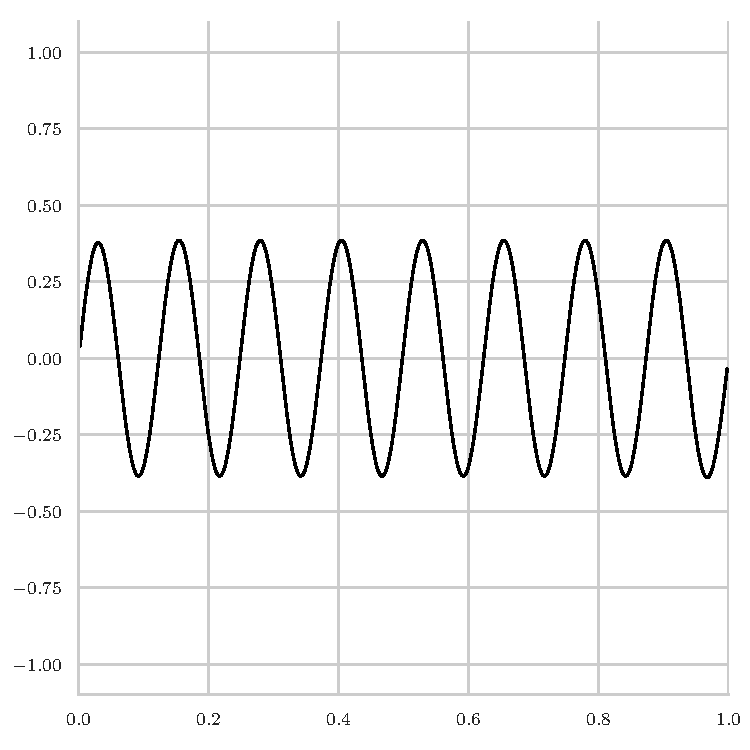
\includegraphics[width=\textwidth]{figures/final_error_gauss_seidel_16pi.pdf}
		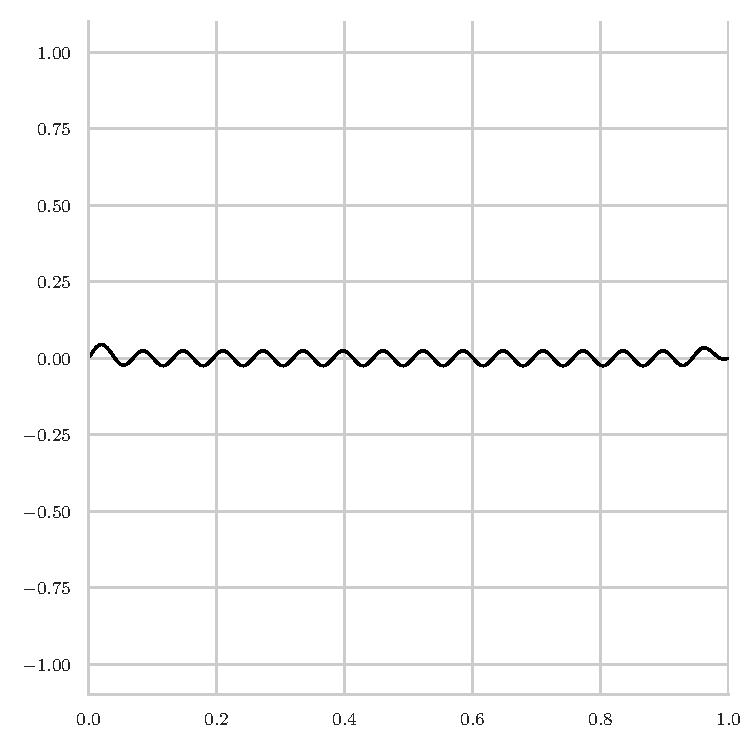
\includegraphics[width=\textwidth]{figures/final_error_gauss_seidel_32pi.pdf}
	\caption{Error after applying Gauss-Seidel}
	\end{subfigure}
	\caption{Different error components on a grid with step size $h = 2^{-9}$ before and after applying either 100 steps of the Jacobi or Gauss-Seidel method.}
	\label{fig:different-error-components}
\end{figure}
Here, the left column shows the initial error discretized on a grid with step size $h = 2^{-9}$ while the middle and right one includes the remaining error after applying 100 Jacobi and Gauss-Seidel steps, respectively.
Note that the frequency of change increases from top to bottom, whereas the amplitude of the error is always the same.
As it becomes apparent from investigating the middle and right columns of the first row of Figure~\ref{fig:different-error-components}, the Jacobi and Gauss-Seidel methods are both not able to achieve a significant reduction of those error components with a low frequency of change within 100 iterations.
In contrast, the third row, which represents a highly-oscillating component, the application of 100 steps of the Jacobi method already reduces the initial error to less than one-fifth of its original value.
The same behavior can also be observed for the Gauss-Seidel method, whereby, compared to the Jacobi method, high-frequency error components are reduced even faster.

We can further illustrate the error reduction properties of basic iterative methods by investigating Figure~\ref{fig:combined-error} which shows the combination of two error components with equal magnitude, one of them with low the other one with high frequency.
Again, the left plot shows the initial while the middle and right ones contain the reduced error after 100 iterations of Jacobi and Gauss-Seidel, respectively.
As it can be seen here, the attained improvement with both methods can be almost fully attributed to the reduction of the highly-oscillating component.
\begin{figure}
	\begin{subfigure}[b]{0.32\textwidth}
	\centering
		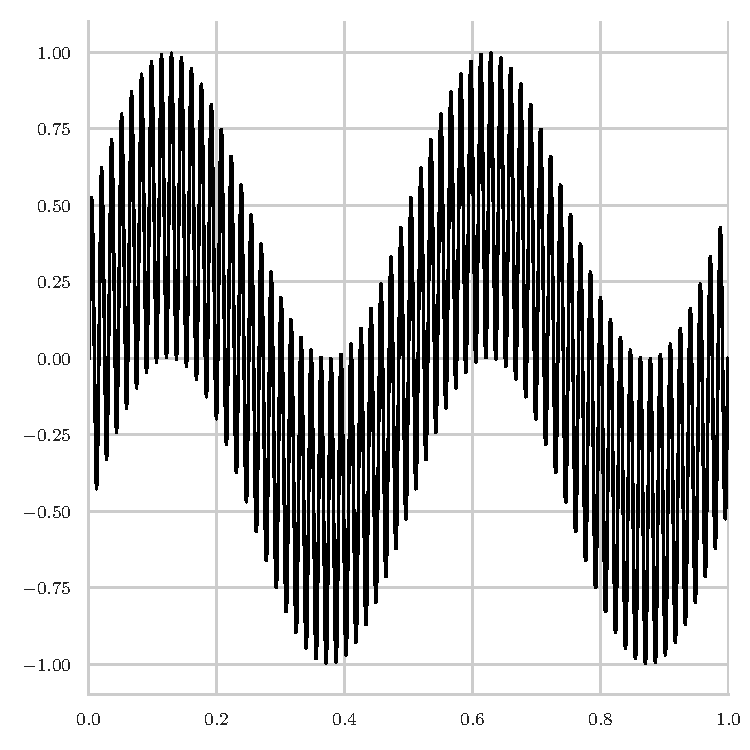
\includegraphics[width=\textwidth]{figures/initial_error_jacobi_combined.pdf}
		\caption{Initial error}
\end{subfigure}
\hfill
\begin{subfigure}[b]{0.32\textwidth}
	\centering
		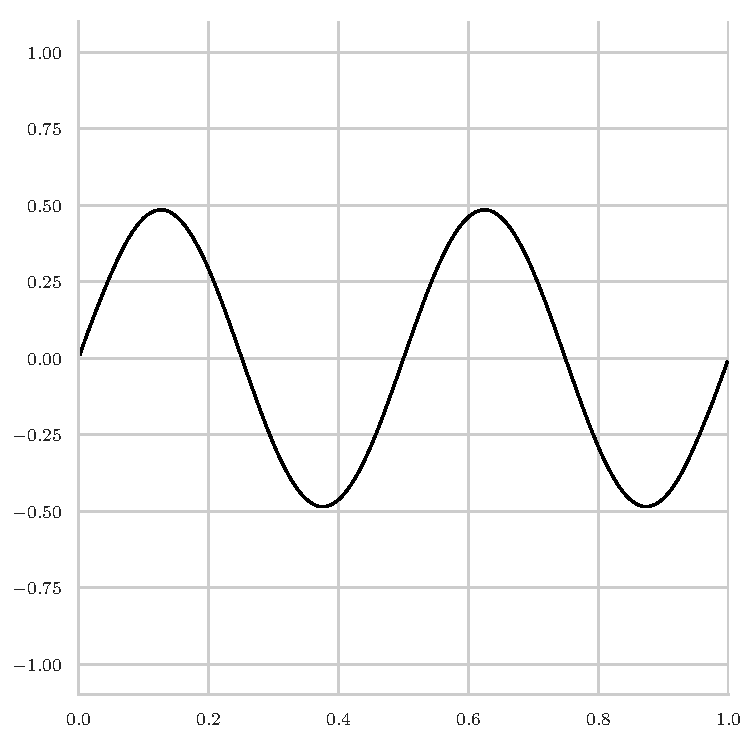
\includegraphics[width=\textwidth]{figures/final_error_jacobi_combined.pdf}
		\caption{Error after applying Jacobi}
\end{subfigure}
\begin{subfigure}[b]{0.32\textwidth}
	\centering
	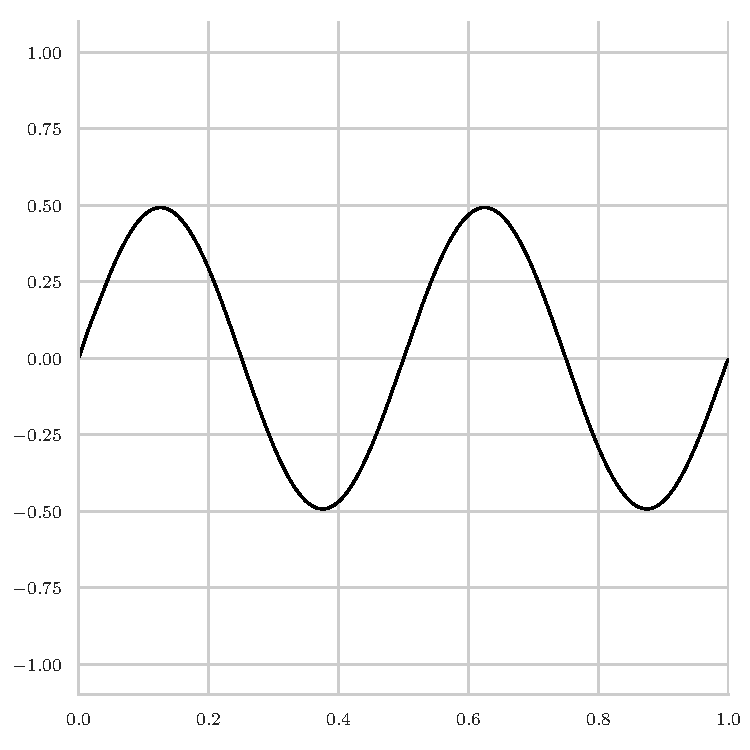
\includegraphics[width=\textwidth]{figures/final_error_gauss_seidel_combined.pdf}
	\caption{Error after applying Gauss-Seidel}
\end{subfigure}
	\caption{Combination of two error components discretized on a grid with step size $h = 2^{-9}$ before and after applying 100 steps of either the Jacobi or Gauss-Seidel method.}
\label{fig:combined-error}
\end{figure}
Because the remaining error is more smooth than initially, basic iterative methods are often denoted as \emph{smoothers} and their effectiveness is measured in terms of their capability to reduce the high-frequency components of a given error. 

Now observe what happens if we represent the same low-frequency error component shown in the first row of Figure~\ref{fig:different-error-components} on a grid with larger step size $h = 2^{-6}$, hence a smaller number of grid points.
Because the number of (inner) grid points $n$ is inversely proportional to the step size with $n = 1/h - 1$, usually the term \emph{coarser} grid is used.
The resulting error reduction, again after 100 iterations of each of both iterative methods, is shown in Figure~\ref{fig:low-frequency-error-component-coarse}. 
\begin{figure}
	\begin{subfigure}[b]{0.32\textwidth}
	\centering
	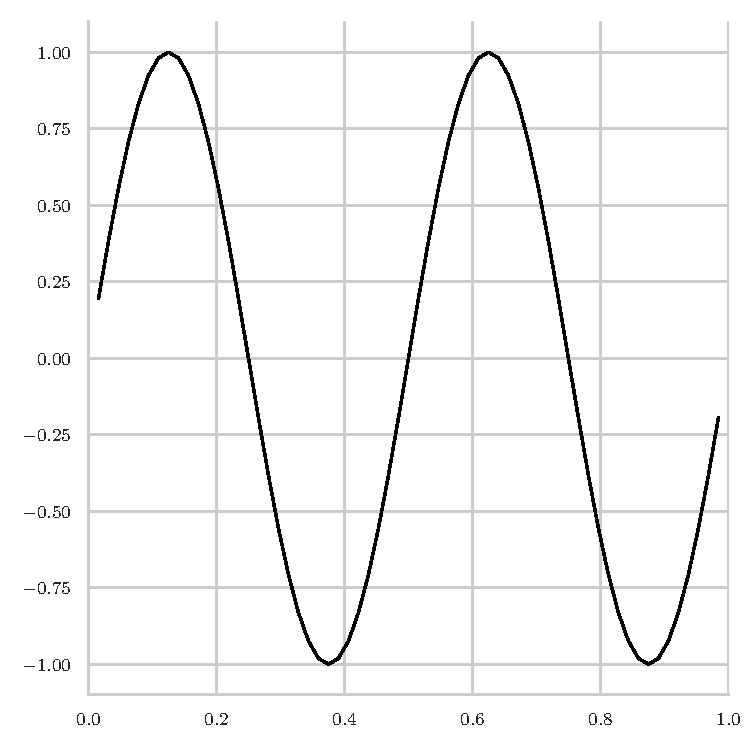
\includegraphics[width=\textwidth]{figures/initial_error_jacobi_4pi_coarse.pdf}
	\caption{Initial error}
\end{subfigure}
\hfill
\begin{subfigure}[b]{0.32\textwidth}
	\centering
	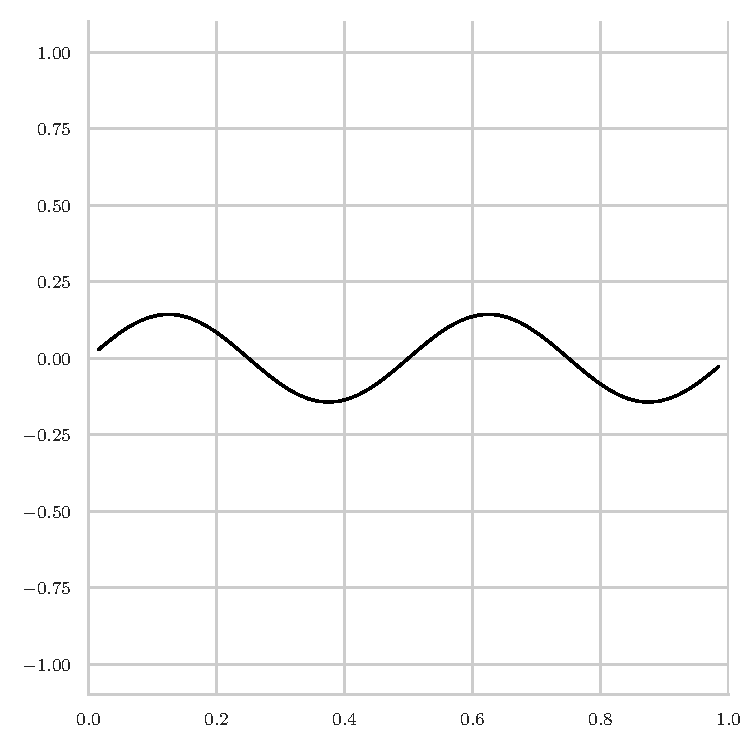
\includegraphics[width=\textwidth]{figures/final_error_jacobi_4pi_coarse.pdf}
	\caption{Error after applying Jacobi}
\end{subfigure}
	\hfill
	\begin{subfigure}[b]{0.32\textwidth}
		\centering
		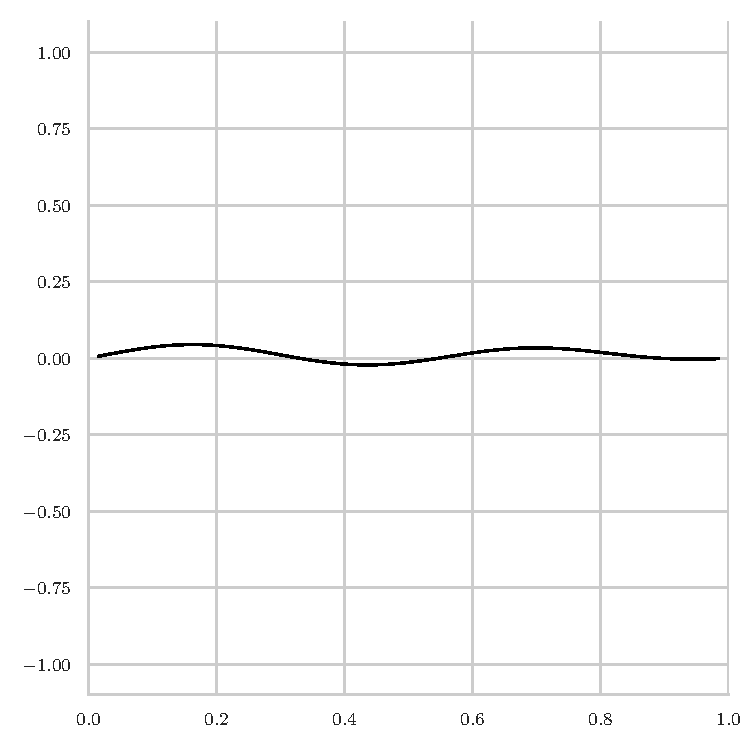
\includegraphics[width=\textwidth]{figures/final_error_gauss_seidel_4pi_coarse.pdf}
		\caption{Error after applying Gauss-Seidel}
	\end{subfigure}
	\caption{Low-frequency error component discretized on a coarse grid with step size $h = 2^{-6}$ before and after applying 100 steps of either the Jacobi or Gauss-Seidel method.}
	\label{fig:low-frequency-error-component-coarse}
\end{figure}
As it can be seen, the amount of low-frequency error reduction is significantly higher for both methods than on the \emph{finer} grid with a step size of $h = 2^{-9}$.
While basic iterative methods, like the Jacobi and Gauss-Seidel method are only capable of reducing the high-frequency components of a given error, we can, hence, employ the same methods to effectively reduce the remaining low-frequency components when they can be represented on a coarser grid.
\emph{Multigrid} methods build up on this idea by automating the process of recursively obtaining a coarser representation of a given problem, which can then be effectively reduced by employing only a few \emph{smoothing} iterations.
These methods, therefore, operate on a so-called hierarchy of grids, where on each subsequent discretization level certain error components are reduced, which is then used to correct the remaining error on the next-finer grid.
In the following, we first introduce the basic components of a multigrid method, such as the smoothing, restriction, prolongation and coarse grid correction operations.
Based on this definition, we then develop a formal language for the representation of multigrid solvers.
\subsection{Smoothing}
One of the central elements of multigrid methods is the utilization of a smoothing procedure, that is able to quickly reduce the oscillatory components of a given error.
We have already shown that the Jacobi and Gauss-Seidel method behave in such a way for the considered one-dimensional model problem.
To further improve the smoothing property of a basic iterative methods, it is often beneficial to introduce an additional relaxation factor $\omega$ which yields the iteration 
\begin{equation}
	\bm{x}^{(i+1)} = \bm{x}^{(i)} + \omega M^{-1}(\bm b - A \bm{x}^{(i)}).
	\label{eq:general-weighted-stationary-iterative-method}
\end{equation}
Again, a weighted Jacobi or Gauss-Seidel can then be obtained by replacing the matrix $M$ by the respective term.
\subsubsection{Red-Black Gauss-Seidel}
While the Gauss-Seidel method exhibits superior smoothing properties compared to the Jacobi method, each iteration requires solving a lower triangular system of the form
\begin{equation*}
	(D - L) (\bm{x}^{(k+1)} - \bm{x}^{(k)}) = \bm{b} - A \bm{x}^{(k)},
\end{equation*}
with $D - L$ as the lower triangular part of the system matrix $A$.
Since $U = A - (D - L)$, we can rewrite this equation to obtain
\begin{equation*}
	(D - L) \bm{x}^{(k+1)} = \bm{b} - U \bm{x}^{(k)}.
\end{equation*}  
which can then be solved using forward substitution by applying
\begin{equation}
	x_{i}^{(k+1)}={\frac {1}{a_{ii}}}\left(b_{i}-\sum _{j=1}^{i-1}a_{ij}x_{j}^{(k+1)}-\sum _{j=i+1}^{n}a_{ij}x_{j}^{(k)}\right),
	\label{eq:gauss-seidel-element-wise}
\end{equation}
where $x_{i}^{(k)}$ represents the $i$th element of the vector $\bm{x}^{(k)}$.
However, because $x_{i+1}^{(k)}$ depends on $x_{i}^{(k)}$ this computation can must be performed sequentially, which means that the individual components of $\bm{x}^{(k+1)}$ must be computed one after another. 
Modern compute architectures exhibit an ever increasing degree of parallelism and, therefore, rely on the fact that all computations can be performed fully in parallel.
For comparison, consider the Jacobi method as defined by 
\begin{equation*}
	\bm{x}^{(k+1)} = \bm{x}^{(k)} + D^{-1}(\bm b - A \bm{x}^{(k)}).
\end{equation*}
Similar to the Gauss-Seidel method, we can first rewrite this equation to
\begin{equation*}
	\bm{x}^{(k+1)} = D^{-1}(\bm b - (A - D)\bm{x}^{(k)}),
\end{equation*}
which then yields the following element-wise formulation of the Jacobi method:
\begin{equation}
x_{i}^{(k+1)}={\frac {1}{a_{ii}}}\left(b_{i}-\sum _{j\neq i}a_{ij}x_{j}^{(k)}\right).
	\label{eq:jacobi-element-wise}
\end{equation}
In contrast to Equation~\eqref{eq:gauss-seidel-element-wise} the computation of each subsequent element of the vector $\bm{x}^{(k+1)}$ does not depend on any of its previous ones.
Consequently, the computation of a new approximate solution $\bm{x}^{(k+1)}$ using the Jacobi method can be performed in parallel for each individual element of the vector.

One possibility to enable a parallel computation of the approximate solution $\bm{x}^{(k+1)}$ that is similar to the Gauss-Seidel method but does not rely on a sequential computation, is to partition the grid points into multiple subsets.
The computation of each subset is then performed in a Jacobi-like fashion, however, in case the values of grid points from other subsets are needed, the updated values are used.
A common variant of this approach is the red-black Gauss-Seidel method.
Here, the grid points are assigned to two distinct sets, where the first represents the red and the second one the black points.
We can define the red-black Gauss-Seidel method in the following way:
\begin{equation}
	\begin{split}
		\bm{x}^{(k+1/2)} & = \bm{x}^{(k)} + P_r D^{-1} (\bm{b} - A \bm{x}^{k}) \\
		\bm{x}^{(k+1)} & = \bm{x}^{(k+1/2)} + P_b D^{-1} (\bm{b} - A \bm{x}^{k+1/2})
	\end{split}
\end{equation}
The entries of the matrices $P_R$ and $P_B$ are then defined as
\begin{equation}
	P_{R,ij} = \begin{cases}
	1 & \text{if} \; i = j \; \text{and} \; i,j \in R \\
	0 & \text{otherwise},  
	\end{cases}
\end{equation}
\begin{equation}
	P_{B,ij} = \begin{cases}
		1 & \text{if} \; i = j \; \text{and} \; i,j \in B \\
		0 & \text{otherwise}  
	\end{cases}
\end{equation}
Here, $R$ and $B$ are the sets of grid indices that correspond to the red and black points, respectively.
Now consider again the three-point stencil defined in Equation~\eqref{eq:1D-laplace-stencil}.
If we define the Gauss-Seidel method with respect to this stencil we obtain
\begin{equation*}
	x_{i}^{(k+1)}=\frac {1}{2}\left(b_{i} + x_{i-1}^{(k+1)} + x_{i+1}^{(k)}\right).
\end{equation*}
Here the update of each individual grid point is exclusively based on its neighbors, whereas the left neighbor $x_{i-1}^{(k+1)}$ has been already updated in the previous step of the method.
We can achieve a similar behavior by assigning neighboring grid points to different partitions, for instance in case of a red-black partitioning by defining
\begin{equation}
		R = \{ \bm{i} : \bm{i} \in \mathbb{N}^d, \sum_{k=1}^d i_k \; \text{even} \}, \;
		B = \{ \bm{i} : \bm{i} \in \mathbb{N}^d, \sum_{k=1}^d i_k \; \text{odd} \}.
\end{equation}
The resulting method can often achieve better smoothing properties as the Jacobi method, without sacrificing much of its parallelism, as the computations on each partition can be performed in parallel.
As an example the effect of one hundred steps of both Gauss-Seidel variants on a combination of different error components is shown in Figure~\ref{fig:combined-error-dominant-high-frequency}.
\begin{figure}
	\begin{subfigure}[b]{0.32\textwidth}
		\centering
		\includegraphics[width=\textwidth]{figures/initial_error_jacobi_dominant_high_frequency.pdf}
		\caption{Initial error}
	\end{subfigure}
	\hfill
	\begin{subfigure}[b]{0.32\textwidth}
		\centering
		\includegraphics[width=\textwidth]{figures/final_error_gauss_seidel_dominant_high_frequency.pdf}
		\caption{Error after applying GS}
	\end{subfigure}
	\hfill
	\begin{subfigure}[b]{0.32\textwidth}
		\centering
		\includegraphics[width=\textwidth]{figures/final_error_red_black_gauss_seidel_dominant_high_frequency.pdf}
		\caption{Error after applying RB-GS}
	\end{subfigure}
	\caption{Combination of three error components with dominant high-frequency term discretized on a grid with step size $h = 2^{-9}$ before and after applying 100 steps of either the Gauss-Seidel (GS) or red-black Gauss-Seidel (RB-GS) method.}
	\label{fig:combined-error-dominant-high-frequency}
\end{figure}


 
%The fundamental requirement of this approach then is that the structure of the matrix $A$ enables a creation of distinct grid point subsets, such that the access
%It is obtained by partitioning the elements of the vector $\bm{x}^{(k+1)}$ into two sets, where the first one represents the set of grid points with an even index, whereas the other one contains those with an odd index.
%TODO describe why RB-GS is only applicable in certain cases 



